\documentclass[10pt,twocolumn]{article}
\usepackage[margin=0.75in]{geometry}
\usepackage{amsmath,amssymb}
\usepackage{booktabs}
\usepackage{graphicx}
\usepackage{xcolor}
\usepackage{siunitx}
\usepackage{hyperref}
\usepackage{cleveref}
\hypersetup{colorlinks=true,linkcolor=blue!50!black,citecolor=green!40!black,urlcolor=blue!50!black}
\usepackage{enumitem}
\usepackage{tikz}
\usetikzlibrary{positioning,calc}
\setlist{nosep,leftmargin=*}
\sisetup{group-separator={,},group-minimum-digits=4}

% TODO markers are kept visible in the draft.
\newcommand{\todo}[1]{\textcolor{red}{[TODO: #1]}}

\title{\textbf{RouteVoice}: A Hardwired-Codebook Speech Recognizer\\in Open 180\,nm Silicon, Built with AI Coding Agents}
\author{Sanjay Prasad H S}
\date{}

\begin{document}
\maketitle

\begin{abstract}
We present RouteVoice, a speech-hardware research implementation targeting open 180\,nm silicon. Its K64 representation encodes 31.46\,M eligible weight positions as fixed 4-bit indices into local UINT8 codebooks. A projection engine selects shared radix-16 partial products, with local register copies across ten lane groups; the recognizer retains INT8 frontend weights, FP32 affine operations and mutable state.

On a reserved 80-utterance test with an additional noisy condition, the quantized Moonshine Tiny model stays within $+2$ WER points of the original by point estimate; confidence intervals exceed that margin in two conditions. Seven converted RTL weight services shrink from \SI{28.64}{MB} to \SI{17.50}{MB}; including five unchanged tables gives \SI{26.34}{MB} of accounted storage. Full-recognizer RTL reproduces the frozen K64 reference's tokens and 18 intermediate hashes on three clips.

A separate $1280\times320$ projection engine (\num{409600} MACs) is routed in GF180MCU. It passes routing, main-deck DRC, LVS, XOR and antenna checks, and meets setup and hold at \SI{150}{ns} across nine PVT/RC corners. Electrical-limit violations remain. Routed power estimated from a zero-delay speech-activity trace is \SI{0.188}{W}, or \SI{287}{pJ}/MAC, excluding its index array. Separately generated banks for 98 matrices occupy \SI{174.7}{mm^2}, with selected-rule DRC and model readback on all banks and full LVS on six representatives.

This is an RTL and open-flow physical-design milestone, not a fabricated or integrated real-time recognizer. We document the evidence, failures and AI-assisted workflow, including \$34.82 of rented compute, and distinguish prospective extensions from demonstrated results.
\end{abstract}

\section{Introduction}
\label{sec:intro}

Voice interfaces can process audio remotely or locally. Local processing can reduce network dependence and keep audio on the device, but requires computation and storage within its power and area budget. For a model fixed over a product's lifetime, mask-programmed weights offer a way to avoid off-chip fixed-weight transfers. Local readout, activation storage and arithmetic still consume energy.

Hardwired, or ``model-specific'', inference silicon has recently attracted commercial attention at the frontier, where fixed-weight chips promise very high token rates for large language models~\cite{taalas2026hc1}. This paper asks the complementary question at the other end of the scale:
\begin{quote}
\emph{Can a useful speech model be hardwired into an open, mature, low-cost process, and can a very small team build and verify it using AI coding agents and open-source tools?}
\end{quote}

We present RouteVoice, a Moonshine Tiny speech recognizer~\cite{jeffries2024moonshine} designed for GlobalFoundries' open 180\,nm process (GF180MCU). Eligible matrices use fixed 4-bit indices into local codebooks. Their integer projection products are assembled from shared partials; frontend INT8 storage, FP32 operations and dynamic attention remain.

The building blocks are not new:
\begin{itemize}
\item codebook-indexed weights~\cite{han2016eie,zadeh2022mokey};
\item shared multiples of an input selected per fixed coefficient~\cite{park2002cshm}, which hardwired-LLM patents also describe~\cite{taalas2025patent802,taalas2026patent566};
\item hardwired weights on an open PDK~\cite{pai2026ankhdjet}.
\end{itemize}
What we add is their combination in a speech recognizer verified at RTL, plus a separately routed projection engine and model-derived index banks. Full-chip physical integration remains incomplete.

\paragraph{Contributions.}
\begin{enumerate}
\item \textbf{A hardwired-codebook weight format, validated for ASR.} K64 stores each weight as a 4-bit index into a 16-entry UINT8 book shared by 64 weights. It keeps Moonshine Tiny within $+2$ WER points of the original on a reserved test, and cuts storage of seven converted RTL services by 39\% (not total model storage).
\item \textbf{A bit-exact recognizer.} The full recognizer RTL decodes speech to the exact tokens and intermediate hashes of the frozen software model, with codebook services, an affine INT8 frontend and unchanged supporting tables.
\item \textbf{A routed, signoff-checked projection engine.} The $1280\times320$ engine (409,600 MACs per projection) closes timing at \SI{150}{ns} in all nine PVT/RC corners. Routing, Magic DRC, KLayout DRC, antenna and LVS checks are clean. Estimated activity-annotated routed energy is \SI{287}{pJ}/MAC; slew, capacitance and fanout violations remain.
\item \textbf{Full-design evidence.} Composed per-module synthesis for silicon and FPGA completes with weight ROMs black-boxed. Mask-programmed banks passing selected DRC checks cover all 98 matrices (\SI{174.7}{mm^2}), with full LVS on six representative banks.
\item \textbf{A documented agent-driven methodology.} We report the step-by-step procedure, the failures and their fixes, and the cost (\$34.82 of cloud compute plus a laptop), and derive concrete practices for faster flows.
\item \textbf{An analysis of future scope.} We size what the same approach implies for local LLMs, and propose ways to make hardwired silicon serve multiple tasks.
\end{enumerate}

\Cref{sec:background} reviews related work. \Cref{sec:representation,sec:architecture} describe the weight format and architecture, and \cref{sec:method} the methodology. \Cref{sec:results,sec:closure} report results, including a timing-closure case study. \Cref{sec:efficiency,sec:future,sec:limitations} discuss efficiency, future scope and limitations.

\section{Background and Related Work}
\label{sec:background}

\paragraph{Hardwired and model-specific inference silicon.}
Fixing a network's coefficients in hardware is old: bespoke printed classifiers hardwire model coefficients and cut area and power by an order of magnitude~\cite{mubarik2020printed}. ROM-based compute-in-memory keeps weights in dense mask ROM and adds a small SRAM path for adaptation:
\begin{itemize}
\item YOLoC~\cite{chen2022yoloc} and Hidden-ROM~\cite{chen2022hiddenrom} do this for CNNs;
\item ROMA~\cite{wang2025roma} puts a quantized LLM base model in ROM and keeps LoRA weights and the key/value cache in SRAM.
\end{itemize}

At the frontier, Taalas has announced HC1, which builds Llama~3.1~8B into a single die and reports about 17k tokens/s per user~\cite{taalas2026hc1,zota2026heise}; these are vendor figures. Its patent applications describe two mechanisms closely related to ours:
\begin{itemize}
\item one multiplier per possible weight value, with a mask-configured mesh routing products to accumulators~\cite{taalas2025patent802};
\item weights stored as hardware pointers into small codebooks~\cite{taalas2026patent566}, alongside a shared-connection mask ROM~\cite{taalas2025wo724}.
\end{itemize}
HNLPU~\cite{liu2025hnlpu} studies the economics of hardwiring a 120\,B-parameter model at \SI{5}{nm}, embedding weights in metal topology to share most mask layers across chips. Etched's transformer-specific ASIC~\cite{mann2024etched} specialises to an architecture class rather than to one set of weights.

Closest to our setting, Ankhdjet~\cite{pai2026ankhdjet} compiles BitNet~b1.58 ternary weights into the via mask of a compute-in-ROM macro on SKY130 and signs it off with open tools. Our work is therefore \emph{not} the first hardwired-weight design on an open PDK. It differs in scope: a complete encoder--decoder speech recognizer, rather than one matrix macro, verified from audio to tokens. It also differs in mechanism: 4-bit codebook indices selecting shared radix-16 partial products, rather than ternary ROM sensing.

\paragraph{Codebook quantization and shared products.}
Storing 4-bit indices into a 16-entry table goes back to Deep Compression~\cite{han2016deepcompression} and its accelerator EIE~\cite{han2016eie}. Mokey~\cite{zadeh2022mokey} applies 4-bit dictionaries to transformers. Modern LLM quantizers explore richer codebooks: AQLM~\cite{egiazarian2024aqlm}, QuIP\#~\cite{tseng2024quipsharp}, VPTQ~\cite{liu2024vptq} and GPTVQ~\cite{vanbaalen2024gptvq} use vector codebooks, and SqueezeLLM~\cite{kim2024squeezellm} uses non-uniform scalar look-up tables. Our K64 format is a scalar non-uniform quantizer of this last kind.

Forming multiples of an input once and selecting them per fixed coefficient is also established:
\begin{itemize}
\item \textbf{DSP:} computation-sharing multipliers~\cite{park2002cshm}, multiplierless multiple-constant multiplication~\cite{voronenko2007mcm} and distributed arithmetic~\cite{white1989da};
\item \textbf{software:} LUT-GEMM~\cite{park2024lutgemm} and T-MAC~\cite{wei2025tmac} apply the same idea to quantized LLMs on GPUs and CPUs;
\item \textbf{run-time weight reuse:} UCNN~\cite{hegde2018ucnn} groups computation by repeated weight values while the network runs.
\end{itemize}
Our datapath combines these known pieces: per-group 16-entry books, radix-16 partial products shared by 320 lanes, and indices fixed at fabrication. We claim the combination and its verified implementation, not the pieces.

\paragraph{Speech recognition hardware.}
Moonshine~\cite{jeffries2024moonshine} is an encoder--decoder ASR transformer whose encoder cost scales with audio length. It reports lower compute than Whisper~\cite{radford2022whisper} tiny at equal error rate, and later variants add streaming encoders~\cite{kudlur2026moonshinev2}.

Dedicated ASR chips have used WFST and DNN--HMM decoders~\cite{price2015wfst,price2018speech} or attention accelerators within an SoC~\cite{tambe2021sm6}, and identified memory bandwidth as the dominant power cost. Always-on keyword-spotting chips reach sub-microwatt power~\cite{shan2020kws,giraldo2018laika}, but only by restricting the task to a few words. RouteVoice targets open-vocabulary transcription and removes weight fetch altogether.

\paragraph{Transformer accelerators and energy references.}
Programmable transformer processors at 12--28\,nm report efficiencies in the tens of TOPS/W~\cite{tu2022trancim,wang2022transformer28nm,tambe2023transformer12nm}. Groq~\cite{abts2020tsp} and Cerebras~\cite{lie2023cerebras} keep weights in on-chip SRAM at scale. Microcontroller NPUs~\cite{arm2024ethosu55,st2024stm32n6} are the commercial baseline for edge voice.

Energy per operation is strongly node- and voltage-dependent~\cite{horowitz2014energy,sze2017tutorial}. Our \SI{180}{nm}, \SI{3.3}{V} figures should be compared with these only after normalisation (\cref{sec:results}).

\paragraph{Open silicon and AI-driven design.}
Our flow builds on the following open tools:
\begin{itemize}
\item OpenROAD~\cite{ajayi2019openroad} and OpenLane~\cite{shalan2020openlane}, now continued as LibreLane~\cite{librelane};
\item Yosys~\cite{wolf_yosys}, Magic~\cite{edwards_magic}, KLayout~\cite{koefferlein_klayout}, Netgen~\cite{edwards_netgen} and Verilator~\cite{snyder_verilator};
\item the open GF180MCU PDK~\cite{google_gf180mcu}.
\end{itemize}
Low-cost shuttles such as Tiny Tapeout~\cite{venn2024tinytapeout} and wafer.space~\cite{waferspace} make fabrication on open nodes affordable.

LLMs have been applied to RTL generation~\cite{liu2023verilogeval,liu2024rtlcoder,chang2023chipgpt}, domain assistance~\cite{liu2023chipnemo}, and flow orchestration~\cite{he2024chateda,jiang2024iicpilot,wang2025mcp4eda,lu2025autoeda}. One accumulator CPU designed through conversation reached tape-out~\cite{blocklove2023chipchat}. Recent studies evaluate coding agents on complete RTL-to-GDS flows~\cite{deng2026rtl2gds} and use them to improve OpenROAD itself~\cite{ghose2026audopeda}. These studies use benchmark-scale designs. We contribute an experience report: a multi-agent team carrying a $10^7$-parameter-class accelerator through physical design, with its failure modes and costs recorded.

\section{Weight Representation}
\label{sec:representation}

\subsection{Model}
We use Moonshine Tiny Streaming (English)~\cite{jeffries2024moonshine}, a 34\,M-parameter encoder--decoder ASR transformer. It has width 320, six encoder and six decoder layers, eight heads of dimension 40, and a 32,768-token vocabulary with tied embedding and output head. Its audio frontend has no FFT or mel stage. Per 5\,ms group of 80 samples it applies:
\begin{enumerate}
\item mean and variance normalisation;
\item an $\operatorname{asinh}$ compression;
\item a learned $80{\to}320$ projection;
\item two stride-2 convolutions, giving 50\,Hz features.
\end{enumerate}
The released model is already integer-quantized (UINT8 weights with per-column zero points and FP32 scales). Our representation starts from those integer weights.

\subsection{K64: four-bit indices into local codebooks}
Each weight matrix is partitioned into groups of 64 consecutive input rows for one output column. A group stores:
\begin{itemize}
\item a book of 16 UINT8 representative values;
\item one 4-bit index per weight, selecting a representative.
\end{itemize}
\begin{figure}[t]
\centering
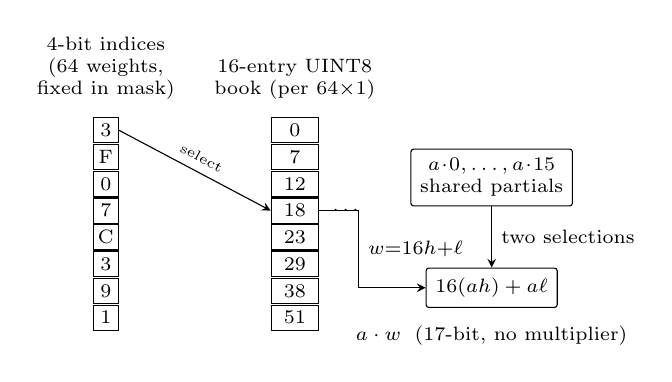
\begin{tikzpicture}[font=\scriptsize,>=stealth,
  box/.style={draw,rounded corners=1pt,minimum height=5mm,align=center},
  cell/.style={draw,minimum width=3.2mm,minimum height=3.2mm,inner sep=0}]
% index column (64 rows shown as 8 cells)
\foreach \i/\v in {0/3,1/F,2/0,3/7,4/C,5/3,6/9,7/1}{
  \node[cell] (i\i) at (0,-\i*0.34) {\v};}
\node[above=1mm of i0,align=center] {4-bit indices\\(64 weights,\\fixed in mask)};
% book
\foreach \j/\v in {0/0,1/7,2/12,3/18,4/23,5/29,6/38,7/51}{
  \node[cell,minimum width=6mm] (b\j) at (2.4,-\j*0.34) {\v};}
\node[right=0.5mm of b3,anchor=west] {\dots};
\node[above=1mm of b0,align=center] {16-entry UINT8\\book (per 64$\times$1)};
\draw[->] (i0.east) -- (b3.west) node[midway,above,sloped]{\tiny select};
% partials
\node[box,minimum width=17mm] (pp) at (4.9,-0.6) {$a\!\cdot\!0,\dots,a\!\cdot\!15$\\shared partials};
\node[box] (add) at (4.9,-2.0) {$16(a h)+a\ell$};
\draw[->] (b3.east) -- ++(0.5,0) |- node[pos=0.25,right]{$w{=}16h{+}\ell$} (add.west);
\draw[->] (pp) -- node[right]{two selections} (add);
\node[below=1mm of add] {$a\cdot w$ \;(17-bit, no multiplier)};
\end{tikzpicture}
\caption{K64 weight representation. Each weight is a fixed 4-bit index into a 16-entry UINT8 book shared by 64 weights of one output column. The selected value's two nibbles select two entries from a 16-entry table of partial products of the current activation $a$. That table is computed once and shared by all 320 lanes.}
\label{fig:k64}
\end{figure}

We call this format K64 (\cref{fig:k64}). Across the model it yields 98 packed matrices, \num{31457280} four-bit selections (\SI{15.7}{MB} of indices) and \num{491520} books.

Because the books hold UINT8 values, the representation slots into the existing integer pipeline unchanged. Zero-point correction, FP32 scaling and bias are applied exactly as in the source graph. The integer weights the chip computes with are \emph{defined} by the books, and our hardware is bit-exact with respect to this frozen K64 model, not the original weights. In the selected $1280\times320$ projection, \num{291832} of the \num{409600} weights differ from the original.

\paragraph{Accuracy.}
Accuracy was settled before any hardware work, under a pre-registered protocol. Candidates were tuned on calibration data, checked once on a development split, and then evaluated once on a reserved LibriSpeech-derived test set~\cite{panayotov2015librispeech}: 80 utterances from 40 held-out speakers, plus a \SI{10}{dB} white-noise copy of the clean set. The gates were an absolute WER ceiling and at most $+2$ points over the original model in each condition.

\begin{table}[t]
\centering\small
\caption{Word error rate (WER) of K64 versus the original Moonshine Tiny on the single reserved test.}
\label{tab:wer}
\begin{tabular}{@{}lrrr@{}}
\toprule
Condition & K64 WER & $\Delta$ vs.\ original & 95\% CI of $\Delta$\\
\midrule
clean & 4.49\% & $+0.23$ & $[-0.83, +1.48]$\\
other & 13.63\% & $+0.89$ & $[-1.51, +3.19]$\\
noise (10\,dB) & 15.77\% & $+1.84$ & $[-0.77, +4.48]$\\
\bottomrule
\end{tabular}
\end{table}

K64 passes all three gates (\cref{tab:wer}). The paired speaker-cluster bootstrap intervals for ``other'' and ``noise'' extend beyond $+2$ points, so we read this as a point-estimate pass on a small test, not a population guarantee. Coarser alternatives failed the same gates: per-tensor 4-bit, 32-column grouped, and K128 (books shared by 128 rows). The per-tensor and grouped candidates lost up to $+9.4$ points on noisy speech.

\subsection{Shared partial products}
\label{sec:shared}
The engine never multiplies a weight. Write each 8-bit representative as $w = 16h + \ell$ with $h,\ell\in[0,15]$. Then
\begin{equation}
a\cdot w = 16\,(a\cdot h) + a\cdot \ell .
\end{equation}
For each input activation $a$ (signed 9-bit), the engine forms the 16 products $a\cdot 0,\dots,a\cdot 15$ once, as 13-bit values. Every one of the 320 output lanes then needs only two selections from this table, a shift and an add to obtain $a\cdot w$; the result fits in 17 bits.

The fixed index picks the book entry, the book entry's nibbles pick two partial products, and the multiply becomes wiring plus a small adder. This mirrors the shared-product idea described in hardwired-weight patents~\cite{taalas2026patent566,taalas2025patent802}. We implement it independently from the public documents, and make no claim about any production implementation.

\subsection{What is fixed, and what is not}
In a fabricated RouteVoice, every 4-bit index is fixed by the mask. Our physical bank uses four mask-programmed access transistors per selection, with the bit pattern set by Via1 positions, followed by a precharged read path per bit. We read the bit pattern back from the GDS and checked it against the packed model.

The books, zero points, scales and biases are fixed constants in the current RTL. Activations, attention state, the audio window and decoder caches are mutable and need SRAM. The measured index bank costs \SI{5.54}{\micro m^2} per selection, including readout and local wiring, against about \SI{51}{\micro m^2} per bit for the open GF180 SRAM macro. Storing every weight in open SRAM would take roughly \SI{6400}{mm^2}; the 81 index banks need \SI{174.7}{mm^2}.

\section{Architecture}
\label{sec:architecture}

\subsection{The projection engine}
The unit of physical work is one $1280\times320$ projection: the decoder feed-forward output matrix, the largest shape in the model. \begin{figure*}[t]
\centering
\resizebox{\textwidth}{!}{%
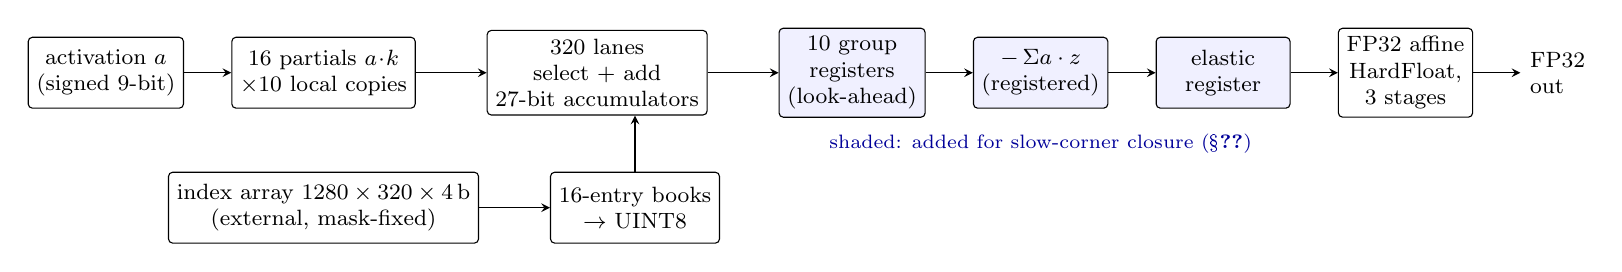
\begin{tikzpicture}[font=\footnotesize,>=stealth,node distance=6mm,
  box/.style={draw,rounded corners=1.5pt,minimum height=9mm,minimum width=17mm,align=center,inner sep=3pt},
  new/.style={box,fill=blue!6}]
\node[box] (in) {activation $a$\\(signed 9-bit)};
\node[box,right=of in] (pp) {16 partials $a\!\cdot\!k$\\$\times$10 local copies};
\node[box,right=9mm of pp] (lanes) {320 lanes\\select $+$ add\\27-bit accumulators};
\node[new,right=9mm of lanes] (grp) {10 group\\registers\\(look-ahead)};
\node[new,right=of grp] (corr) {$-\,\Sigma a\cdot z$\\(registered)};
\node[new,right=of corr] (pipe) {elastic\\register};
\node[box,right=of pipe] (fp) {FP32 affine\\HardFloat,\\3 stages};
\node[box,below=8mm of pp] (arr) {index array $1280\times320\times4$\,b\\(external, mask-fixed)};
\node[box,right=9mm of arr] (book) {16-entry books\\$\to$ UINT8};
\draw[->] (in)--(pp); \draw[->] (pp)--(lanes);
\draw[->] (arr)--(book); \draw[->] (book.north) -- (book.north |- lanes.south);
\draw[->] (lanes)--(grp); \draw[->] (grp)--(corr); \draw[->] (corr)--(pipe); \draw[->] (pipe)--(fp);
\draw[->] (fp.east) -- ++(6mm,0) node[right,align=left]{FP32\\out};
\node[below=2mm of corr,font=\scriptsize,text=blue!60!black] {shaded: added for slow-corner closure (\S\ref{sec:closure})};
\end{tikzpicture}}
\caption{The $1280\times320$ projection engine. The index array sits outside the engine's physical top. One projection takes 4,165 cycles: 1,280 rows of LOAD/INDEX/ACCUM, one PREP cycle, 320 output cycles and four pipeline-fill cycles.}
\label{fig:engine}
\end{figure*}

The engine (\cref{fig:engine}) is a five-state machine:
\begin{description}
\item[LOAD] accepts one signed 9-bit activation, adds it to a running activation sum, and registers its 16 partial products.
\item[INDEX] reads one 1,280-bit row of the index array (320 four-bit selections) and maps each index through its book to a UINT8 representative.
\item[ACCUM] adds, in each of 320 lanes, the two selected partial products (one shifted) into a signed 27-bit accumulator.
\item[PREP] (added in \cref{sec:closure}) fills per-group output registers before output begins.
\item[OUTPUT] emits one column per cycle. Each value is the accumulator minus $\text{activation sum}\times\text{zero point}$, passed through a three-stage FP32 multiply--add (Berkeley HardFloat~\cite{hauser_hardfloat}) that applies the activation scale, the weight scale and the bias with independent round-to-nearest-even steps.
\end{description}
One projection takes $3\times1280$ cycles of LOAD/INDEX/ACCUM and 320 output cycles, plus pipeline fill: 4,165 cycles in the final design (4,163 originally). That is 409,600 multiply-accumulates, an average of 98 MAC per cycle.

Two structural changes made the engine physically implementable:
\begin{enumerate}
\item \textbf{Fanout.} Row-index and partial-product nets originally drove up to \num{11359} loads. We duplicated the row registers ten times and capped synthesis fanout at 16.
\item \textbf{Local partials.} Each 32-lane group gets its own copy of the partial-product registers, so the 208-bit partial-product bus no longer crosses the die (\cref{sec:closure}).
\end{enumerate}
Both changes are cycle-identical on the full test bench.

\subsection{From one engine to a recognizer}
The full recognizer RTL connects:
\begin{itemize}
\item the PCM input and frontend;
\item the six-layer encoder;
\item an adapter that produces cross-attention keys and values;
\item a greedy six-layer decoder that ends at the end-of-sequence token.
\end{itemize}
Everything runs on one common clock. Each weight service answers lookups through index and book ROMs. The top level has no weight inputs: its 31 runtime inputs are audio, clocks, resets, handshakes and configuration.

\paragraph{Throughput.}
A dense one-pass estimate of the workload is about 0.6\,GMAC/s:
\begin{itemize}
\item the encoder: about 7.4\,M MAC per frame at 50 frames/s;
\item the decoder: about 21.5\,M MAC per token at about 4 tokens/s;
\item the keys and values produced for cross-attention.
\end{itemize}
One engine at \SI{150}{ns} sustains 0.66\,GMAC/s. However, the native streaming controller re-processes encoder frames and regenerates cross-attention keys and values. Measured on real traces, that controller needs 10--90 engine-equivalents at a \SI{120}{ns} clock. Real-time operation therefore depends as much on scheduling as on raw MAC rate, and we treat it as open (\cref{sec:limitations}).

\subsection{Chip plan}
All 98 matrices map to 81 pitch-matched index banks (\SI{174.7}{mm^2}) plus four bank-driver control strips (\SI{56.6}{mm^2}). Abstract floorplans with power grids give two candidate chips:
\begin{itemize}
\item \textbf{One die} of $25\times31$\,mm, which needs a denser SRAM than the open GF180 macro (we assumed \SI{12}{\micro m^2}/bit);
\item \textbf{Two dies} of $25\times29$\,mm, built only from existing open parts, with no change to the numerics.
\end{itemize}
The two-die variant routes and passes IR drop at the measured engine power, but fails an earlier, more pessimistic assumed-load IR screen.

About 1.09\,MB of mutable state (activation banks, key/value caches, history and scratch) dominates the remaining area. Synthesized as flip-flops, it alone puts the logic at \SI{1198}{mm^2} (\cref{sec:results}). Mapping it onto SRAM macros is the largest open area item.

\section{Methodology}
\label{sec:method}

\subsection{Proof levels and evidence rules}
Every claim in the project names an artifact and a proof level. The levels run from P0 (idea) through software, numerical reference, RTL block, connected RTL, open-flow physical design, FPGA, foundry signoff and silicon, up to P9 (product). A claim at one level never stands in for another. A routed engine is not evidence of recognizer accuracy, and a correct index pattern is not evidence of a correct weight.

Three rules governed the work:
\begin{enumerate}
\item A result is recorded as PASS only after the lead re-ran it or read the actual tool output. Reports from worker agents are recorded as ``claimed'' until then.
\item Failures are kept, not overwritten. Each workstream keeps a \texttt{FAILURES.md} next to its \texttt{RESULTS.md}.
\item Inputs and outputs are pinned by SHA-256: model tensors, packed indices, books, tool binaries and run databases. Off-machine backups are re-hashed after upload.
\end{enumerate}

\subsection{Step-by-step procedure}
\begin{enumerate}
\item \textbf{Freeze the model and the oracle.} Pin the Moonshine release by hash. Build an independent NumPy reference over the executable tensor bytes, and capture boundary tensors, logits and tokens for each test clip.
\item \textbf{Choose the representation in software.} Search quantization candidates against pre-registered WER gates, ending with one reserved test (\cref{sec:representation}).
\item \textbf{Write a numerical contract for one projection.} Fix bit widths, cycle counts and an exact integer and FP32 oracle. Bound accumulators on the actual matrix.
\item \textbf{Build and verify the RTL engine.} The bench uses 54 vectors: one captured from speech and 53 integer fixtures, giving \num{17280} integer and \num{17280} FP32 outputs. It also exercises stalls and four mid-vector resets.
\item \textbf{Connect the whole recognizer.} Move every weight on chip, first as byte ROMs, then with eligible services converted to index$+$book storage. Require identical tokens, hashes and clock counts on every change.
\item \textbf{Lay out the weight banks.} Generate pitch-matched mask-programmed banks. Then run DRC, read the bit pattern back from GDS against the packed model, and run LVS against a source-derived netlist. Include planted-error negative controls.
\item \textbf{Implement the engine physically.} Synthesize, audit fanout, run short global-route diagnostics, then do the full route, signoff (DRC, LVS, antenna, XOR) and all-corner extracted timing.
\item \textbf{Estimate power from real activity.} Run a gate-level simulation of one real projection, rescale its switching trace to the clock period, and annotate it on the routed database with extracted parasitics.
\item \textbf{Check whole-design synthesizability} for both silicon and FPGA.
\item \textbf{Floorplan the chip} with abstract macros, power grids and IR-drop screens, then attempt partial integration of real banks and logic macros while recording unresolved stubs and connectivity.
\end{enumerate}

\subsection{Open toolchain}
All tools are open source:
\begin{itemize}
\item \textbf{Synthesis:} Yosys~0.62~\cite{wolf_yosys}, including \texttt{slang} for SystemVerilog.
\item \textbf{Place and route:} OpenROAD~\cite{ajayi2019openroad} under LibreLane~3.0.11~\cite{librelane}.
\item \textbf{Timing:} OpenSTA~2.7.
\item \textbf{Layout and DRC:} Magic~8.3~\cite{edwards_magic} and KLayout~0.30~\cite{koefferlein_klayout}, using the full GF180 main deck.
\item \textbf{LVS:} Netgen~1.5~\cite{edwards_netgen}.
\item \textbf{Circuit simulation:} ngspice~47.
\item \textbf{Functional and gate-level simulation:} Verilator~5.05~\cite{snyder_verilator}.
\end{itemize}
The PDK is GF180MCU-D~\cite{google_gf180mcu} with its 7-track standard cells, characterised at TT (\SI{25}{\celsius}, \SI{3.3}{V}), SS (\SI{125}{\celsius}, \SI{3.0}{V}) and FF (\SI{-40}{\celsius}, \SI{3.6}{V}), each with minimum, nominal and maximum RC. The toolchain is pinned in a Nix environment.

Compute was an Apple M4~Pro laptop (14 cores, 48\,GB) and two rented CPU servers. The servers were used for about 47 hours in total and cost \$34.82. All closure and power work after 22~October ran on the laptop.

\subsection{Agent orchestration}
The design work was carried out by AI coding agents under human direction:
\begin{itemize}
\item a lead agent (Claude Code) planned the work, wrote briefs, verified results and integrated them;
\item up to six parallel worker agents (OpenAI Codex CLI) each owned one workstream, with a written brief, a private directory, and explicit limits on compute, memory and cloud spend;
\item short-lived sub-agents handled read-only research and inventories.
\end{itemize}

Workstreams in the final push were:
\begin{itemize}
\item W10: engine routing and signoff;
\item W11: index$+$book recognizer;
\item W12: full synthesis;
\item W13: weight banks;
\item W14: logic macros;
\item W15: two-die integration.
\end{itemize}

The human set goals and budgets and approved spending. The lead enforced the evidence rules. Several practices proved necessary:
\begin{itemize}
\item \textbf{Verify process state, not worker reports.} Workers sometimes reported jobs as ``continuing'' after their processes had exited. One such case left a rented server idle for about 21 billed hours.
\item \textbf{Publish a shared resource schedule.} A container's real memory limit (\SI{64}{GB}) was far below what the operating system reported (\SI{755}{GB}). After one out-of-memory kill, the lead published a priority order and a memory ceiling for all workers.
\item \textbf{Keep a verified external backup before tearing down cloud machines.} A 53\,GB checksum-verified backup let the rented server be deleted while results were still being produced; routed power and every later closure run started from the restored data.
\item \textbf{Have the lead do the critical-path engineering.} Timing closure (\cref{sec:closure}) ran as short, verified iterations by the lead after the workers had exited. This was the recorded working practice, not a controlled comparison of delegation strategies.
\end{itemize}
\Cref{sec:efficiency} quantifies where time and money went.

\section{Results}
\label{sec:results}

We report three kinds of evidence, in decreasing order of completeness:
\begin{itemize}
\item functional bit-exactness of the whole recognizer;
\item a separately routed projection engine with scoped physical checks;
\item synthesizability of the whole recognizer for both silicon and FPGA.
\end{itemize}
The review reconciles the paper with archived reports and tool metrics; it does not rerun the silicon flow. Source files and their scopes are listed in \cref{app:artifacts}.

\subsection{Bit-exact recognition from index and codebook weights}
The full recognizer RTL decodes the clip ``Switch on the lights'' to the token sequence $[28176, 373, 278, 26068, 2]$. Eligible services use 4-bit indices into local 16-entry books; the frontend retains affine INT8 weights and supporting tables remain unchanged. All 18 checked output hashes match the reference, and the run takes \num{312578649} clocks, identical to the earlier byte-ROM design. Two further clips (``Plant present.'' and ``Seasonable.'') also match on all 18 hashes.

\Cref{tab:storage} covers the seven services converted in W11. Their storage falls from \SI{28.64}{MB} to \SI{17.50}{MB} ($-38.9\%$); decoding reproduces all \num{28641280} bytes of the frozen K64 byte-ROM baseline, not the original source model. Five unchanged tables add \num{8847360} bytes, giving \num{26344960} accounted bytes. Small LUTs and mutable state are excluded. The separate full-model software export and its 31.46\,M indexed positions have a different scope and must not be equated with this incremental RTL conversion. Exhaustive RTL checks of the lookup responders cover \num{565960} encoder/decoder packets, \num{2074560} frontend packets and \num{163840} position packets.

The test set is small. It establishes that the hardware representation is \emph{exact} with respect to the quantized model, not that the quantized model is accurate. Accuracy of the codebook quantization itself was measured in software on held-out speech (\cref{sec:representation}).

\begin{table}[t]
\centering\small
\caption{Storage of the seven converted W11 services, followed by unchanged tables. Decimal bytes; small LUTs and mutable state excluded.}
\label{tab:storage}
\begin{tabular}{@{}lr@{}}
\toprule
Component & Bytes\\
\midrule
4-bit indices (\num{78970880} bits) & \num{9871360}\\
16-entry UINT8 books (one per 64 weights) & \num{4935680}\\
Affine INT8 frontend (lossless) & \num{2073600}\\
Metadata (scales, zero points, biases) & \num{616960}\\
\midrule
Converted subtotal & \num{17497600}\\
Five unchanged tables & \num{8847360}\\
\midrule
Accounted total & \textbf{\num{26344960}}\\
\bottomrule
\end{tabular}
\end{table}

\subsection{Routed projection engine}
The $1280\times320$ engine top contains the arithmetic and output stages for \num{409600} four-bit selections. The fixed index array sits outside it and is supplied by the test bench. Physical design used LibreLane on GF180MCU-D (7-track cells, 5 metal layers) at \SI{150}{ns}.

The final design is ``fix~2'' in \cref{sec:closure}, after an antenna close-out pass. On a \SI{22.84}{mm^2} die it has \num{1146232} standard cells (54.0\% utilization) and \SI{68.9}{m} of routed wire. Signoff results:
\begin{itemize}
\item detailed routing: zero violations;
\item Magic DRC: zero violations;
\item KLayout DRC (main GF180 deck): zero violations;
\item GDS XOR between the Magic and KLayout streams: zero differences;
\item antenna: zero violating nets or pins;
\item LVS (Netgen): circuits match uniquely, with zero device, net, pin or property differences.
\end{itemize}
Setup and hold are met in all nine PVT/RC corners; the slowest is SS with worst-case RC at $+8.10$\,ns, and the worst hold slack is $+0.32$\,ns. The final metrics still report worst-corner counts of \num{902948} max-slew, \num{24390} max-capacitance and \num{30058} max-fanout violations. Passing setup and hold does not clear these electrical limits; complete signoff remains open.

Each projection takes 4,165 cycles, so one engine at \SI{6.67}{MHz} sustains about \SI{0.66}{GMAC/s}. This exceeds only the dense one-pass estimate. The controller's trace-derived 10--90 engine-equivalent demand at \SI{120}{ns} prevents a demonstrated real-time recognizer claim.

\begin{figure*}[t]
\centering
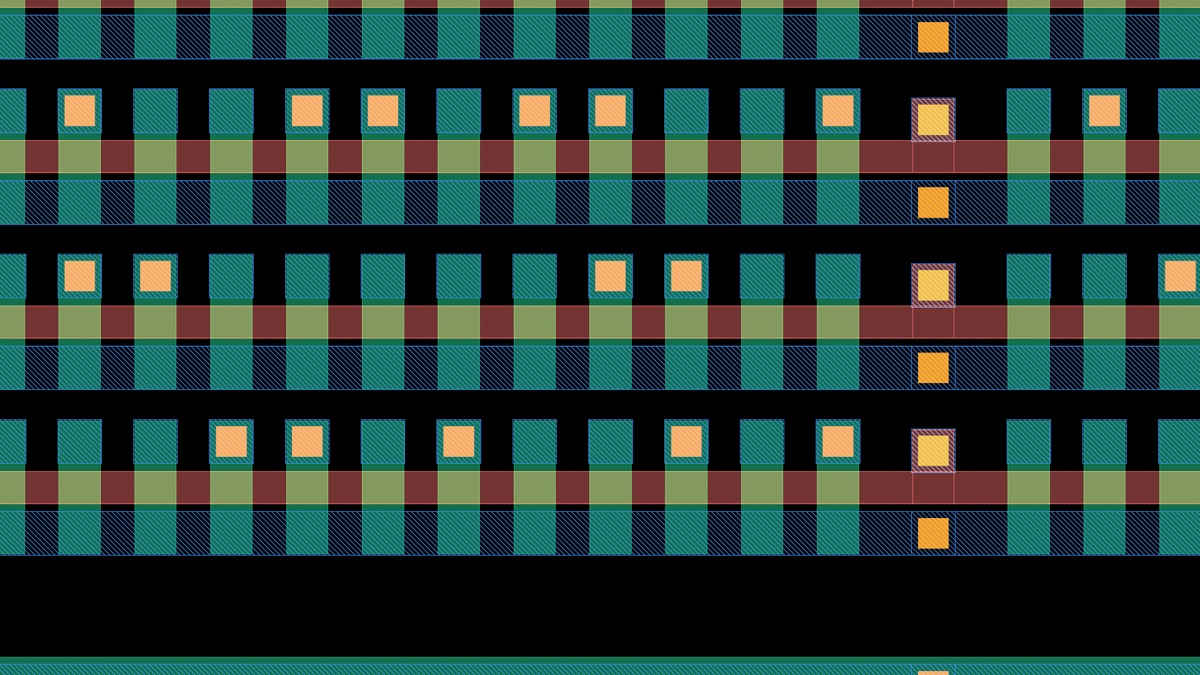
\includegraphics[width=0.49\textwidth]{figures/layout-weight-cells.jpg}\hfill
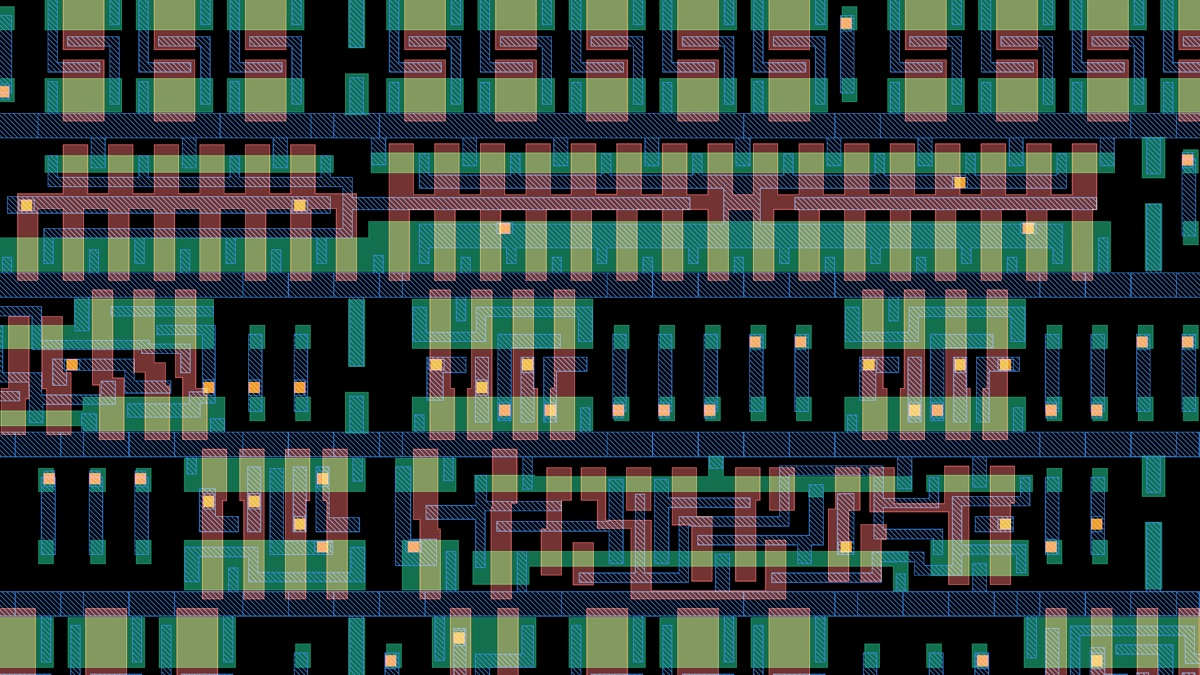
\includegraphics[width=0.49\textwidth]{figures/layout-engine-cells.jpg}
\caption{Layout close-ups rendered from the GDS (Via1 amber, Metal1 blue, poly and diffusion beneath; fill hidden). \emph{Left:} \SI{10.4}{\micro m}-wide window of weight bank \texttt{W13\_ENC0\_B00}. Each 4-bit index uses four mask-programmed access transistors; the irregular Via1 pattern over the regular cell grid sets the stored bits. \emph{Right:} \SI{29.5}{\micro m}-wide window of the routed $1280\times320$ engine (fix~2): standard cells of the select-and-accumulate datapath. Zoom sequences from full die to cells are in the release package (\cref{app:artifacts}).}
\label{fig:layout}
\end{figure*}

\paragraph{Power.}
Activity comes from a zero-delay gate-level simulation of one real-speech projection on the synthesized netlist. All 320 FP32 outputs of that run are bit-exact. Annotated against the final routed database and extracted parasitics, estimated engine power is \SI{0.188}{W} at TT and \SI{150}{ns}: \SI{142}{mW} combinational, \SI{24}{mW} sequential and \SI{21.5}{mW} in the clock tree. That is \SI{117}{\micro\joule} per projection, or \SI{287}{pJ} per MAC.

These are tool estimates, not silicon measurements. There is no matched multiplier-based GF180 baseline, so the result does not establish an energy advantage over conventional MAC hardware. Cross-node operation-energy comparisons~\cite{horowitz2014energy} require matched precision, workload, memory, voltage and physical scope. The flattened power report separates combinational, sequential and clock power, but does not isolate the integer core from FP32 affine logic. A per-module breakdown remains open.

The pre-route estimate for the same engine was \SI{162}{pJ}/MAC; that figure had no clock tree and only placement parasitics. Pin annotation was 67.5\%; the remaining pins are cells inserted after synthesis, which the analyser assigns default activity. The trend across iterations (241$\to$256$\to$287\,pJ/MAC) therefore mixes real design change with falling annotation coverage.

\subsection{Whole-recognizer synthesizability}
Synthesizing the complete recognizer flat failed for both silicon and FPGA. Synthesis tools stalled for hours in memory and flip-flop optimisation passes, and the FPGA run crashed. We therefore black-boxed the weight ROMs and synthesized the remaining 30,545 elaborated modules as 4,457 distinct units, each under a 6\,GB memory limit. All 4,457 units pass for a generic library, for GF180, and for the Lattice ECP5 FPGA family.

These separately synthesized units give an upper-bound-style estimate without cross-boundary optimization or weight-ROM interiors, not a placed or fully integrated netlist. The composed GF180 logic estimate is \SI{1198}{mm^2} (\SI{11.98}{cm^2}) (48.4\,M cells, 8.07\,M flip-flops), because all \num{8169778} bits of mutable state (buffers, caches, normalisation state) become flip-flops when no SRAM macros are inferred. That is $19\times$ the \SI{63}{mm^2} logic budget of our floorplan. The ECP5 mapping needs 30.4\,M LUT4s, 1.34\,M flip-flops, 1,247 DSP blocks and 118 BRAMs, far beyond any device in the family. The seven converted storage services alone (\num{139980800} bits) also exceed on-FPGA memory by more than an order of magnitude.

\subsection{Toward a full chip}
Several physical parts of the full chip exist but are not integrated:
\begin{itemize}
\item \textbf{Weight arrays.} All 98 weight matrices (\num{31457280} selections) are laid out as 81 pitch-matched index banks totalling \SI{174.7}{mm^2}. Every bank passes the selected DRC rules and GDS bit-pattern readback; density and antenna are outside that bank check. Full LVS passes on six representative banks, not all 81. A single bank measures \SI{5.54}{\micro m^2} per selection for its bank-local layout.
\item \textbf{Bank drivers.} Four driver/control shapes pass their selected DRC and LVS checks and meet \SI{150}{ns} across nine corners. Complete capture and array-periphery qualification remains open.
\item \textbf{Logic macros.} Six leaves meet the workstream's local READY criteria, which defer density to chip fill. Supplemental density checks still fail (five or seven markers per leaf); this is not complete block signoff.
\item \textbf{Two-die top level.} Two $25\times29$\,mm outlines contain 48 real banks, four logic leaves and 119 stubs, with bank drivers pending. Only 14 scalar nets are source-matched; 1,368 are synthetic test nets. Top wiring passes its routing checks, but minimum density remains unmet and assumed-load IR fails (VDD/VSS: A 0.869/0.866\,V, B 1.44/1.35\,V). Full-chip DRC completion, LVS and STA remain open; no complete neural datapath is demonstrated.
\end{itemize}
\Cref{sec:limitations} discusses what remains.

\section{Case Study: Closing the Slow Corner}
\label{sec:closure}

\begin{table*}[t]
\centering\small
\caption{Engine closure iterations. Setup slack (worst endpoint) is in ns at a \SI{150}{ns} clock with extracted parasitics. Energy uses activity-annotated routed power at TT. Completed routed runs pass routing, Magic DRC, main KLayout DRC and LVS checks; fix 1 stopped before completion. Electrical-limit violations remain. Antenna counts are open nets after repair.}
\label{tab:closure}
\setlength{\tabcolsep}{4.5pt}
\begin{tabular}{@{}lrrrrrrl@{}}
\toprule
Run & GRT ovf. & TT & SS nom & SS max & Antenna & pJ/MAC & What changed\\
\midrule
First route (var.\ C) & 575 & $-72.9$ & $-251$ & $-307$ & 130 & 241 & local partials; no post-placement repair\\
Closure ECO 1 & -- & $+55.0$ & $-40.0$ & $-55.5$ & 4 & 256 & post-route repair; antenna diodes\\
Closure ECO 2 & -- & $+56.7$ & $-36.2$ & $-53.1$ & 4 & -- & more aggressive repair\\
Fix 1 (stopped) & 3,206 & -- & -- & -- & -- & -- & register before FP32 stage\\
Fix 2 & 9 & $+67.6$ & $+21.6$ & $+8.3$ & 11 & 287 & $+$ split 320:1 select\\
\textbf{Fix 2, final} & \textbf{9} & $\mathbf{+67.5}$ & $\mathbf{+21.4}$ & $\mathbf{+8.1}$ & \textbf{0} & \textbf{287} & $+$ 10 antenna-repair rounds\\
\bottomrule
\end{tabular}
\end{table*}

Timing closure of the $1280\times320$ engine illustrates both how the open flow behaves at scale and why architectural fixes beat tool tuning. \Cref{tab:closure} summarises each iteration. Rows with timing entries use extracted-parasitic (RCX/SPEF) static timing at a \SI{150}{ns} clock (\SI{6.67}{MHz}).

\paragraph{Congestion first.}
The first full placements could not be routed. Global routing reported 3.37\,M overflowed resources, because one set of radix-16 partial products fed all 320 lanes across the die. Giving each 32-lane group its own cycle-identical copy of the partial-product registers (``local partials'') cut overflow to 260\,k, and then to 575 once post-placement repair was disabled. Detailed routing then converged to zero violations.

\paragraph{Tool-level closure plateaus.}
With routing clean, the typical corner (TT, \SI{25}{\celsius}, \SI{3.3}{V}) met timing with $+55$\,ns of slack. The slow corner (SS, \SI{125}{\celsius}, \SI{3.0}{V}) failed by $-40$\,ns (nominal RC) and $-55.5$\,ns (worst-case RC). We ran two engineering-change (ECO) passes, re-entering the flow after global routing. They used more aggressive repair: a \SI{45}{ns} setup-slack margin, buffering allowed up to 50\% of cells, 100\% of failing endpoints targeted, and 20 antenna-repair iterations. These passes recovered only about 4\,ns (to $-36.2$/$-53.1$\,ns), and the \emph{same} 30 endpoints failed in both. We stopped tuning there: the failing paths were too deep for one cycle at SS, whatever the repair settings.

\paragraph{Diagnosis.}
All 30 failing paths start at the column register. They then pass through:
\begin{itemize}
\item the 320:1 accumulator select;
\item the zero-point lookup and its correction multiply and subtract;
\item the integer-to-floating-point conversion.
\end{itemize}
They end in the first register stage of the FP32 affine block.

The two first-order models disagreed on the size of the problem. Using estimated parasitics after global routing, the pre-fix design showed $+36$\,ns of SS slack. Its routed result was $-36$\,ns, a 72\,ns gap. The gap comes from the die-wide 320:1 select: its fan-in wires are long and only appear once detailed routing is done.

\paragraph{Fix~1: one elastic register.}
We first inserted an elastic valid/ready register between the integer engine output and the FP32 affine stage; weight scale, bias and column index move through it with the data. Throughput is unchanged, and latency grows by one cycle (4,163 to 4,164 cycles per projection). The 54-vector bench still matched all 17,280 FP32 outputs bit-exactly. Estimated SS slack on the column path rose from $+36$ to $+61$\,ns. Applying the 72\,ns gap leaves an expected routed slack of about $-10$\,ns, still failing. Global-route overflow also rose to 3,206. We therefore stopped this run at detailed routing.

\paragraph{Fix~2: split the select with look-ahead group registers.}
Each 32-lane group now registers its own lane for the \emph{look-ahead} column, so the output path sees only a 10:1 select of group registers. The look-ahead column is $c{+}1$ on an output handshake and $c$ otherwise. The zero-point correction is registered the same way. A single \texttt{PREP} state between the last accumulation and the first output fills these registers. The change is generated by a script from the original RTL. It adds one more cycle (4,165 per projection), keeps one output per cycle, and again passes all 54 vectors bit-exactly.

The physical effect was large. Global-route overflow fell to 9, and detailed routing converged in about 75 minutes. The completed geometric/equivalence checks report zero routing, Magic and main KLayout DRC violations, a unique Netgen LVS match, and zero GDS XOR differences; 11 antenna nets remain open, against 4 before. All nine corners (TT/SS/FF $\times$ min/nom/max RC) meet setup and hold at \SI{150}{ns}. The worst case is $+8.34$\,ns at SS with worst-case RC, against $-53.1$\,ns before.

\paragraph{Antenna close-out.}
The 11 open antenna nets were not a design problem. The router's post-route antenna repair had stopped at its default three rounds while still converging (199, 41, 24, then 11 violating nets). Re-running from the same detailed-routing input with up to ten rounds, and nothing else changed, took the count to zero: 8, 5, 5, 5, 1, 1, then 0, adding about 1,000 diodes (7,452 in total). The listed open-flow checks were then repeated: routing, Magic and KLayout DRC, XOR, disconnected-pin and power-grid checks are all zero, and LVS again matches uniquely. Timing moved by less than \SI{0.3}{ns} in every corner (worst $+8.10$\,ns setup, $+0.32$\,ns hold), and routed power with the same activity trace is unchanged. The run took 6.7 hours on a laptop, two of them in KLayout DRC.


\paragraph{Cost of closure.}
Routed, activity-annotated power for fix~2 is \SI{0.188}{W} at \SI{150}{ns} at TT. That is \SI{117}{\micro\joule} per projection, or \SI{287}{pJ} per MAC, about 12\% more than the ECO-1 design (\SI{256}{pJ}/MAC). The increase accompanies extra group registers, registered correction and repair buffering; the flattened report cannot assign a measured energy increment to each change. Both power runs annotate about 68\% of pins from a zero-delay gate-level trace of one real-speech projection. The unannotated pins belong to repair, antenna and diode cells that do not exist in the synthesized netlist.

\paragraph{Lesson.}
Two passes of repair-setting tuning, about 17 hours of compute, did not move the failing endpoints. One RTL change of under 40 lines, verified bit-exactly on the full bench within minutes, closed every corner and also removed the routing congestion. The general rule we draw is to pipeline wide selects and long fan-in paths at RTL before physical design. A small set of path-level timing estimates, calibrated against one fully routed run, is enough to decide when to stop tuning.

\section{Making It Faster and More Efficient}
\label{sec:efficiency}

We separate improvements to the \emph{design}, which change area or energy, from improvements to the \emph{flow}, which change how long it takes to reach a verified design.

\subsection{Design}
\paragraph{Map mutable state to SRAM.}
The full-recognizer synthesis infers 8.17\,M mutable bits as flip-flops; the entire composed logic estimate is \SI{1198}{mm^2}. A bridge using 160 open GF180 SRAM macros passes an untimed, mapped protocol replay of deterministic feature words: 20,480 values, 2,560 packets and 511 held cycles over 163,158 clocks. It includes reset and malformed-response cases plus explicit macro pin checks, but no neural arithmetic, extracted timing or physical implementation. Mapping the remaining state, preserving behavior and qualifying the physical memory interfaces remain substantial work.

\paragraph{Time-share datapaths.}
The RTL instantiates separate arithmetic for each service. A small number of projection engines, scheduled over all matrices, would replace most of that logic. The scheduling question is the one raised in \cref{sec:architecture}: how many engine-equivalents real-time streaming really needs.

\paragraph{Lower the activity, not just the clock.}
Combinational logic draws 75\% of engine power (\SI{142}{mW} of \SI{188}{mW}). The 320 accumulators and partial-product selectors toggle on every accumulation cycle. Candidate changes to evaluate are:
\begin{itemize}
\item gate the clock of lanes whose selected product is zero;
\item narrow the accumulators to the bound proven on the actual matrix;
\item operand-isolate the FP32 stage outside the output phase.
\end{itemize}
Savings and timing consequences have not been measured. Each proposal requires functional checks, implementation and activity-based comparison.

\paragraph{Voltage and node.}
The current implementation uses the GF180 \SI{3.3}{V} 7-track library. Typical-corner timing slack alone does not establish operation at a lower supply; that requires characterized libraries and renewed timing, noise and reliability checks. A newer process could improve density and energy, but $CV^2$ intuition~\cite{horowitz2014energy} is not a validated migration model for these arrays and long wires. The area scenarios in \cref{sec:future} are assumptions, not demonstrated energy savings.

\subsection{Flow}
The project's own history shows where the time went and what would have saved it.

\begin{enumerate}
\item \textbf{Route a short diagnostic first.} Three-iteration global-route diagnostics took 25--61 minutes and found the congestion cause. Full routing attempts without that diagnostic burned about 11 hours in global routing and about 1 hour per detailed-routing iteration without converging. Only start a full route once the diagnostic overflow is small: overflow of 575 routed in hours, while 260\,k never did.
\item \textbf{Fix wiring and depth in RTL, not with die area or repair settings.} A die 1.6 times larger cut overflow by only 24\%, while local register copies cut it by 92\% at the same area. Two aggressive repair passes moved slow-corner slack by 4\,ns, while one RTL pipeline change moved it by 58\,ns and reduced overflow from 575 to 9. When the same endpoints fail after repair, pipeline.
\item \textbf{Pick a reachable clock early.} Repairing toward \SI{20}{ns} grew area by 26\% and never finished, because the datapath was about \SI{145}{ns} deep. At \SI{150}{ns} the design closed.
\item \textbf{Audit fanout at synthesis.} Capping fanout at 16 cut estimated power $10.8\times$ and turned placement from hours into minutes.
\item \textbf{Calibrate pre-route timing once.} Estimated slow-corner slack after global routing was 72\,ns optimistic for die-spanning paths. One calibration against a routed result was enough to stop a doomed run early (fix~1) and to predict that fix~2 would close.
\item \textbf{Check that repair loops converged, not just stopped.} The last 11 antenna violations remained only because the router's post-route repair loop ends after three rounds by default, while it was still halving the count each round. Raising the limit to ten cleared them with no design change. Read iteration logs, not just final counts.
\item \textbf{Signoff dominates wall time.} KLayout DRC takes about 2 hours on every run, comparable to detailed routing. Run signoff only on candidates that already meet timing, and parallelise or tile the DRC deck.
\item \textbf{Most of the work fits on a laptop.} The initial routing work used rented compute; later closure and power runs after 22 October ran locally. Those local engine runs took roughly 4--9.5 hours and incurred no additional cloud charges, excluding laptop, electricity and human effort. Whole-design synthesis needed big memory only when attempted flat; per-module synthesis under 6\,GB per process completed every unit.
\item \textbf{Bill only for active compute.} Roughly 21 of the 47 rented hours were idle. An idle-CPU auto-stop, plus checking worker process state rather than worker reports, would have saved over a third of the cloud spend (about \$13 of \$34.82).
\item \textbf{Check format compatibility early.} An activity-file syntax mismatch between simulator and timing analyser, and a cell-name format bug in a buffering script, each cost a full run cycle.
\end{enumerate}

In aggregate, the engine went from its first RTL contract (13--14 October) to a routed, all-corner-closed layout clean on DRC, LVS and antenna checks (24 October) in eleven calendar days, including a five-day pause. The final timing fix, including the abandoned first attempt, took about seven hours from diagnosis to all-corner routed timing.
A two-to-three-day rerun is a retrospective planning estimate, not a measured replication or evidence of an agent speedup against a human-only baseline.

\section{Future Scope: Local LLMs and Multi-Purpose Transformer Silicon}
\label{sec:future}

RouteVoice combines full-recognizer RTL with one separately routed projection engine and separately generated index banks. This section sets out what the same techniques imply for local language models and for silicon that serves more than one transformer. Unlike the rest of the paper, these are projections, not measurements.

\subsection{From recognizer to voice assistant}
A useful local voice device chains speech-to-text, a small language model, and text-to-speech. Transformer-based choices for these stages share dense projections, attention and normalization, but their frontends, state, operators and scheduling can differ.

The projection engine here is model-agnostic below the index fabric. It consumes a stream of signed activations and a fixed table of 4-bit selections, and emits FP32 results. A second model would also require compatible shapes and numerics, new books and metadata, control and state planning, and validation of unsupported operators. Reuse of this projection mechanism is a possibility, not demonstrated multi-model compatibility.

Mutable state is an additional scaling constraint alongside fixed-weight storage, arithmetic and integration. A recognizer's mutable state is its audio window and decoder cache. An autoregressive LLM adds a key/value cache that grows with context, which belongs in SRAM or external DRAM, never in metal.
For scale, a 0.5\,B-parameter LM such as Qwen2.5-0.5B~\cite{qwen2024qwen25,qwen05config} (24 layers, two key/value heads of dimension 64) keeps 6,144 key/value values per token. At 8 bits, a 2,048-token context needs about \SI{12.6}{MB}, roughly twelve times all of RouteVoice's mutable state (8.17\,Mbit).

\subsection{Hardwired weights at larger scale}
Fixed-index storage has a clear scaling trade:
\begin{itemize}
\item \textbf{Benefits:} fixed coefficients need no off-chip weight transfers; local index/book readout still costs energy, and mutable state can still require off-chip bandwidth. This does not establish a security property.
\item \textbf{Cost:} a mask set per model.
\end{itemize}
Commercial hardwired-LLM efforts~\cite{taalas2026hc1} accept that cost at the frontier for throughput.

Our results suggest a complementary point at the low end, and they let us size it.

\paragraph{Throughput.} A dense decoder-only LM of $N$ parameters needs about $N$ multiply-accumulates per generated token. One of our engines sustains \SI{0.66}{GMAC/s} at \SI{6.67}{MHz}. Ignoring attention, state transfers, control, utilization and inter-engine communication gives a MAC-only upper bound of about 1.3 tokens/s per engine, or 13 for ten ideally utilized engines. These are not measured generation rates or demonstrated voice-assistant latency.

\paragraph{Area.} Index area alone is already a major constraint; this calculation excludes compute and mutable state. At our measured \SI{5.54}{\micro m^2} per selection, 0.5\,B selections need about \SI{2800}{mm^2} at \SI{180}{nm}, several reticles.

\paragraph{Node scaling.} Ideal area scaling to \SI{28}{nm} is $(180/28)^2\approx41\times$, which would bring the same banks to roughly \SI{70}{mm^2}. Peripheral circuits scale worse than this, so the figure is an optimistic bound. \Cref{fig:scaling} plots the measured points and an assumed 20--40$\times$ band, without a physical port validating either endpoint.

\begin{figure*}[t]
\centering
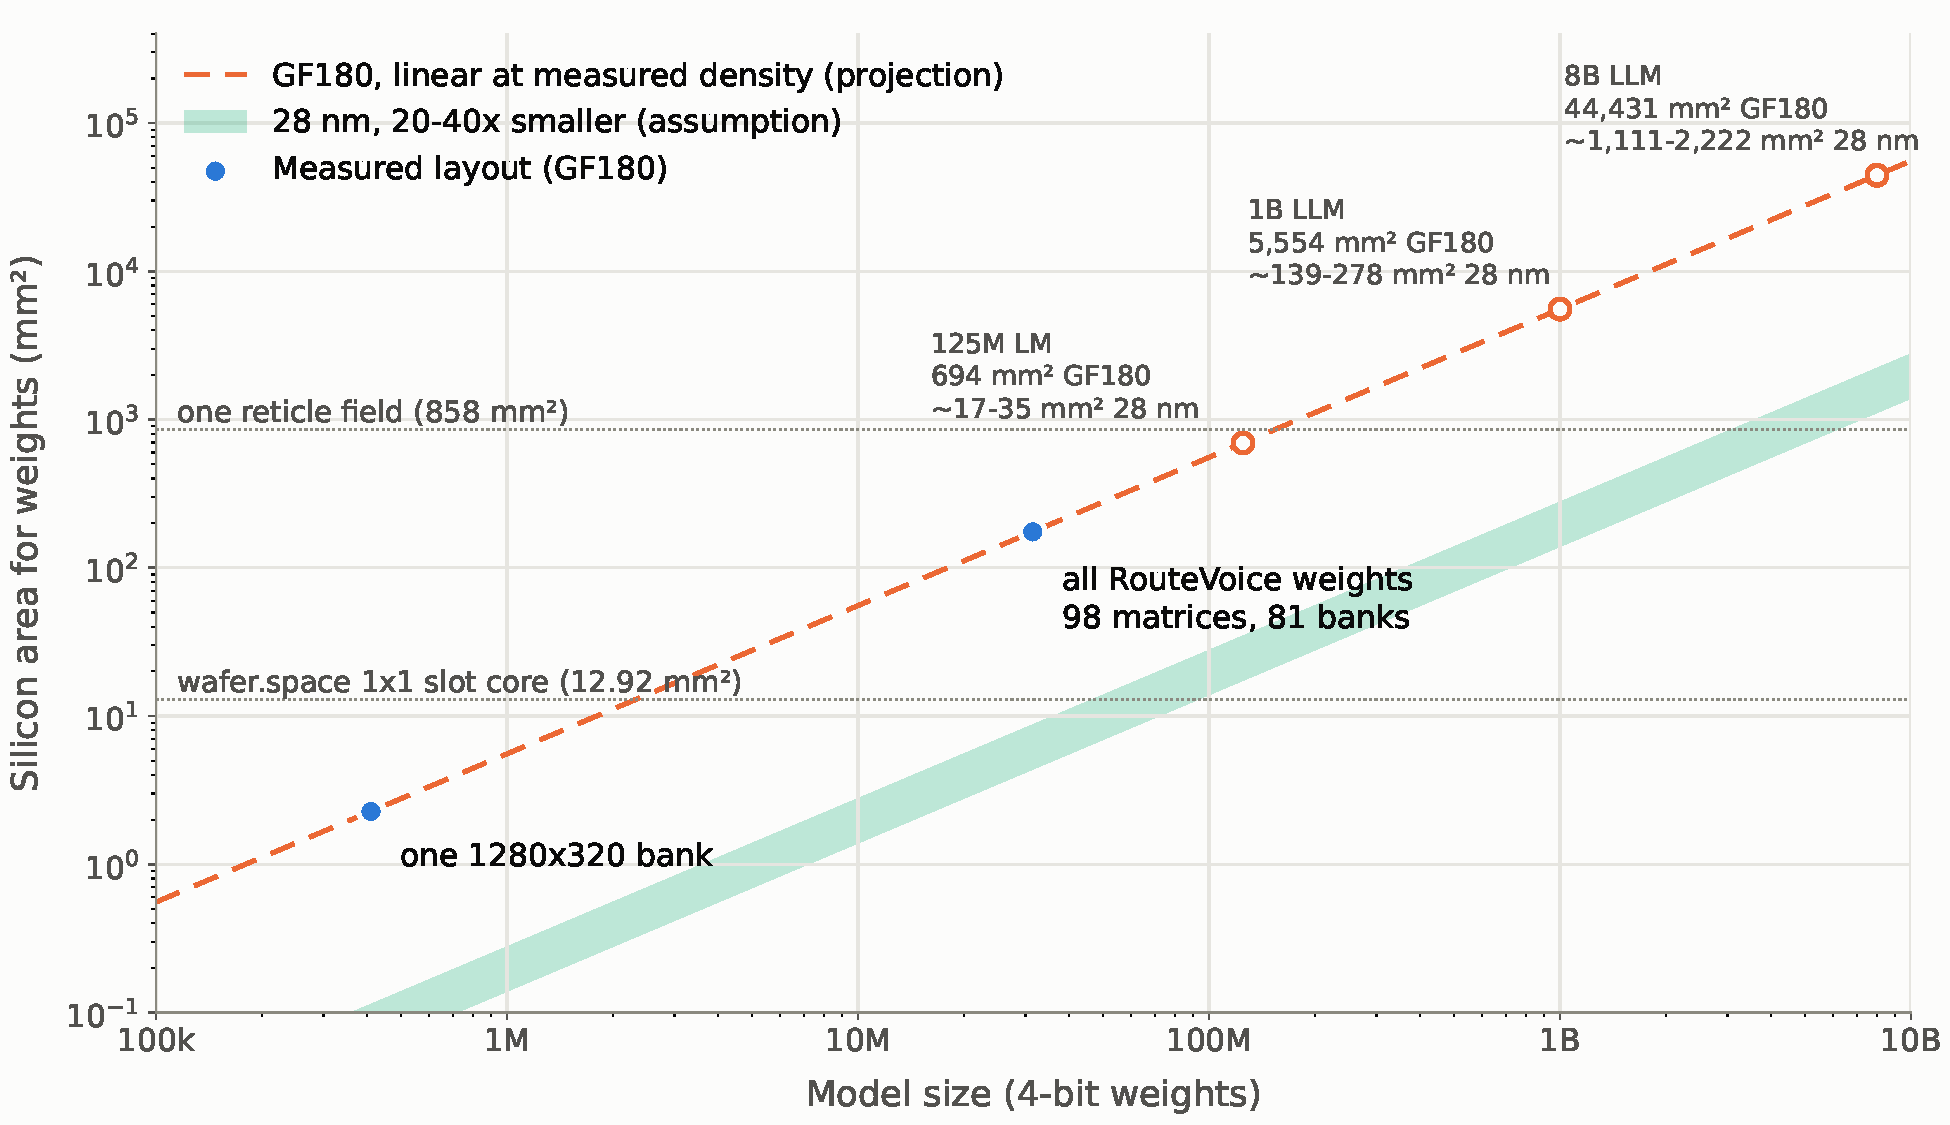
\includegraphics[width=0.8\textwidth]{figures/scaling-area.pdf}
\caption{Weight-array area against model size. Filled points are measured GF180 layout: one $1280\times320$ bank (\SI{2.27}{mm^2}) and all 98 RouteVoice matrices (\num{31457280} four-bit weights, \SI{174.7}{mm^2}, i.e.\ \SI{5.55}{\micro m^2} per weight including readout). The dashed line extends that density linearly; the shaded band assumes a 20--40$\times$ area reduction at \SI{28}{nm}. Both are projections, not measurements. Weights only: compute engines, activation and KV memory, and I/O are excluded.}
\label{fig:scaling}
\end{figure*}

\paragraph{Where this leaves the low end.} This work lays out the fixed indices for a tens-of-millions-parameter speech model on a mature node. It does not establish a complete recognizer fit, yield or cost. A sub-billion-parameter LM would require substantial density improvement before even its fixed indices approach a practical single-die area; affordability also depends on integration and manufacturing economics.

\subsection{Making hardwired silicon multi-purpose}
Hardwiring trades flexibility for efficiency. Several mechanisms can recover flexibility without returning to fully programmable weights:
\begin{enumerate}
\item \textbf{Mutable codebooks over fixed indices.} The 4-bit indices are fixed; the 16-entry books (\SI{4.9}{MB} for the services we converted, about half the index bytes) could instead live in SRAM. Then one die could be re-tuned after fabrication: recalibrated, rescaled, or fine-tuned within the span its fixed indices allow. At open-SRAM density that costs far more area than the books do as ROM, so it suits a model family whose indices are shared and whose books differ. Whether book-only fine-tuning recovers useful accuracy is an experiment we have not run.
\item \textbf{Low-rank adapters in SRAM.} A fixed base model plus small SRAM-resident adapters (LoRA-style) on selected projections supports task or speaker adaptation. The existing 160-SRAM bridge tests memory protocols only; it does not implement or validate LoRA arithmetic or adaptation.
\item \textbf{Shared backbones.} Distilling several tasks onto one shared encoder lets one fixed fabric serve many heads: transcription, keyword spotting, intent, language identification. Only the small task heads stay mutable.
\item \textbf{Family dies.} A mask set can hold several small models whose index fabrics share one engine and I/O ring, selected at run time. Area grows linearly in model bytes, but NRE is paid once.
\end{enumerate}

\subsection{Economics}
The economic case depends on volume, yield, packaging and model lifetime. Open-PDK shuttles~\cite{waferspace} provide a possible route to small test structures, but the current \SI{22.84}{mm^2} engine already exceeds an approximately \SI{20}{mm^2} slot before adding its array and I/O. The two proposed \SI{725}{mm^2} dies are a different manufacturing scale. We have no verified quotation for a complete recognizer and make no affordability claim.

This project documents an AI-assisted design process; it does not measure a causal speedup over a controlled alternative. Potential applications include appliance voice control, wearables and industrial sensors whose model can remain fixed, subject to resolving the energy, timing, quality and integration limits above.

\section{Limitations}
\label{sec:limitations}

We state the boundaries of the evidence explicitly.

\begin{itemize}
\item \textbf{No silicon.} Every physical result comes from open-source tools on an open PDK. None has passed foundry signoff or been fabricated.
\item \textbf{Engine, not chip.} Routing, signoff, timing and power cover one $1280\times320$ projection engine, without its index array. The two-die chip is floorplanned and partly integrated. It has no full-chip DRC, LVS or timing, and it fails an assumed-load IR-drop check.
\item \textbf{Open signoff items.} The final engine is clean on DRC, LVS and antenna checks with the open GF180 decks. Slew, capacitance and fanout-limit violations remain in the final metrics; they cause no setup or hold failure, but a foundry signoff would require them fixed.
\item \textbf{Power fidelity.} Activity comes from one real projection, simulated without delays (so glitches are not modelled), with 67.5\% of pins annotated. The rest are cells added during physical design and receive default activity. Neither fabricated-silicon power nor full-recognizer physical power has been measured.
\item \textbf{Timing simulation.} Post-layout simulation replayed all vectors on the routed netlist without delays. None of the simulators available to us supports SDF timing checks at this scale.
\item \textbf{Real-time operation is unproven.} One engine meets a dense one-pass MAC estimate. The native streaming controller's measured workload needs 10--90 engine-equivalents, and the frontend's per-chunk deadline implies a far higher clock than the engine's. A service schedule that meets real time has not been built.
\item \textbf{Accuracy.} The bit-exact results are against the frozen K64 model. K64's accuracy rests on one reserved test of 80 utterances from 40 speakers, whose confidence intervals cross the $+2$-point gate for noisy and ``other'' speech. Streaming quality on live audio was not measured.
\item \textbf{Scale of RTL.} The composed per-module estimate is \SI{1198}{mm^2}, or \SI{11.98}{cm^2}, for the whole logic scope with mutable state inferred as flip-flops. It excludes ROM-service interiors and cross-boundary optimization; it is neither memory-only area nor a placed chip.
\item \textbf{Array and macro scope.} Bank checks exclude density/antenna and full LVS covers six representatives. Driver/capture integration remains open. W14 leaf density failures and synthetic W15 connectivity prevent treating their local READY labels as full-chip signoff.
\item \textbf{Relation to Taalas.} We implement ideas described in public patent documents. We make no claim about any company's production design.
\end{itemize}

\section{Conclusion}
\label{sec:conclusion}

RouteVoice shows that a real speech transformer can be expressed entirely as fixed 4-bit indices and small codebooks, without leaving the accuracy envelope of its source model. It also shows that the resulting arithmetic engine can be carried through an all-open-source flow to a routed, DRC-clean layout that closes timing in every corner of a 180\,nm process.

The most transferable lessons are methodological. The fixes that mattered were all at RTL: local register copies against congestion, and pipelining a die-wide select against slow-corner timing. They were found fastest by short, calibrated experiments, not by long tool sweeps. AI coding agents made it possible to run many workstreams in parallel at very low cost. They were reliable only when every claim was checked against the tools' own outputs.

The open work is concrete: mapping mutable state to SRAM, scheduling for real time, full-chip signoff, and silicon. Fixed-model silicon at mature nodes, built quickly with open tools and agents, is a credible path to private, low-power voice and language interfaces for everyday devices.


\bibliographystyle{plainurl}
\bibliography{refs}

\appendix
\section{Artifacts}
\sloppy
\label{app:artifacts}

All paths are relative to the RouteVoice repository root, \url{https://github.com/sanjuhs/routevoice}. \path{FIN} denotes \path{routing-voice-chip-design/overnight-20261014/finish-1023}.

\begin{itemize}
\item \textbf{Release package (demo clips, simulation logs, layout renders, signoff table, scaling data):} \path{routing-voice-chip-design/release-v1/}.
\item \textbf{Bit-exact recognizer with index$+$codebook weights:} \path{FIN/w11-taalas-e2e/RESULTS.md}, \path{results.json}.
\item \textbf{K64 accuracy:} \path{routing-voice-chip-design/docs/TAALAS-K64-QUALITY-RESULT.md}.
\item \textbf{Engine contract and bench:} \path{routing-voice-chip-design/overnight-20261014/fabric-k64/CONTRACT.md}, \path{RESULTS.md}.
\item \textbf{Engine routing history:}
  \begin{itemize}
  \item first route: \path{FIN/w10-route/RESULTS.md};
  \item closure passes: \path{FIN/w10-route/closure-lead/};
  \item first-route power: \path{FIN/w10-route/routed-power-lead/}.
  \end{itemize}
\item \textbf{Final engine (fix~2):} \path{FIN/w10-route/pipe2/} (README, generator \path{make_engine.py}, bench, flow configuration, \path{evidence/}; antenna close-out in \path{evidence-ant/}).
\item \textbf{Final engine run backup (fix~2 and antenna close-out, checksum manifests):} Hugging Face dataset \path{sanjuhs/routevoice-engine-fix2-20261024}.
\item \textbf{Full-recognizer synthesis:} \path{FIN/w12-synth/RESULTS.md}.
\item \textbf{Weight banks:} \path{FIN/w13-arrays/RESULTS.md}, \path{DRIVERS-RESULTS.md}.
\item \textbf{Logic macros and two-die integration:} \path{FIN/w14-blocks/}, \path{FIN/w15-chip/}.
\item \textbf{Chronological lab log:} \path{OVERNIGHT-PROGRESS.md}.
\item \textbf{Cloud run backup (53\,GB, checksum manifest):} Hugging Face dataset \path{sanjuhs/routevoice-pod-final-20261022}.
\end{itemize}

\end{document}
